\section{\huge{Bonusopgaver}}

\subsection{Den hyggelige opgave}

Forbind prikkerne.

\begin{center}
\includegraphics[width=.99\textwidth]{forbind-prikkerne.pdf}
\end{center}


\newpage
\subsection{Rus opgaven}
Udtryk funktionen \texttt{fold} udelukkende ved hjælp af
\texttt{foldBack} og uden eksplicit rekursion.
Husk at \texttt{foldBack} og \texttt{fold} i F\# har typerne:

\begin{align*}\small
  \text{foldBack} &: ('T \rightarrow 'State \rightarrow 'State) \rightarrow 'T\ list \rightarrow 'State \rightarrow 'State\\
  \text{fold} &: ('State \rightarrow 'T \rightarrow 'State) \rightarrow 'State \rightarrow 'T\ list \rightarrow 'State
\end{align*}

\subsection{2. års rus opgaven}
Som storkunde hos internetudbyderen IP Factory har du har fået tildelt IP-adresseblokken 200.23.18.0/23.
Hvor mange forskellige IP-adresser råder du over? Angiv også den højeste og den laveste IP-adresse i dit råderum.

\subsection{3. års rus opgaven}
Konstruer en SLR-parsertabel for følgende grammatik:

\[
S \rightarrow \texttt{torben}\ S'\ \texttt{og}\ \texttt{fritz}
\]
\[
S \rightarrow \texttt{torben}\ F\ \texttt{og}\ \texttt{torben}
\]
\[
F \rightarrow S''\ \texttt{fritz}\ S''\ \texttt{fritz}\ S\ |\ \texttt{torben}\ \texttt{, }\ F
\]
\[
S' \rightarrow \epsilon\ |\ \texttt{, }\ S
\]
\[
S'' \rightarrow \texttt{, }\ |\ \texttt{, }\ S\ \texttt{, }
\]

\newpage

\subsection{De små opgaver}
\vspace{-0.1cm}

\subsubsection{Underopgave 0}
\vspace{-0.2cm}

Donald kan godt lide primtal, men kender kun primtallene op til 2. Hjælp ham
ved at lave en F\# (eller SML) funktion, der finder alle primtal under 100.

\subsubsection{Underopgave 1}

Donald elsker IEEE standarder og har for nyligt fundet IEEE 754 til
repræsentation af tal. Hjælp ham med at omskrive tallet $173.8$ til dets
32-bit IEEE 754 repræsentation. Blev der mistet præcision?


\subsubsection{Underopgave 2}
\vspace{-0.2cm}

Implementér en x64-simulator i C.

Husk at indentere med mellemrum og ikke lave for lange linjer.

\subsubsection{Underopgave 3}
\vspace{-0.2cm}

Håndkør følgende Whitespace-program og rapportér dets output:
\begin{verbatim}





\end{verbatim}

\newpage
\subsection{C opgaven}
For at undgå flaskehalse har Kantinebestyrelsen anskaffet sig en ny colaautomat
med et flerbrugersystem, så nu kan $n > 1$ brugere købe cola fra den samme
automat samtidigt.  Automaten blev leveret med følgende enterprise-kode:
\begin{verbatim}
int antal_colaer = 1000;

void køb_en_cola() {
  afspil_fanfare();
  if (antal_colaer > 0) {
    træk_kroner(15);
    antal_colaer--;
    giv_cola();
  }
}
\end{verbatim}
Antag at koden køres samtidigt af flere brugere.  Lokalisér kapløbsstriden og
reparér den med en lås.

\textbf{Diskussion:} Føler du dig bedre rustet til opgaven efter ACS?

\newpage

\subsection{Den skægge opgave}

Mentorerne har bagt pandekager i Kantinen og vil dele ud af dem. De er
dog blevet enige (efter at have set lidt for meget Rasmus Klump) om at de skal
sættes dem i ét tårn. Da de har bagt for mange pandekager er de
dog havnet med et problem; de har ikke sorteret deres tårn efter størrelse,
hvilket forårsager ustabilitet i tårnet.
\begin{center}
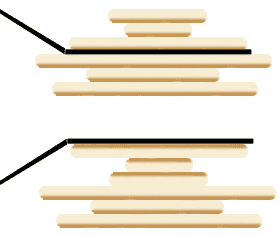
\includegraphics[width=0.48\textwidth]{figures/pandekager.png}
\end{center}
Det er dit job at hjælpe mentorerne med at sortere dem. Til hjælp har du én
spatel, som du kan indsætte et sted i stakken af pandekage og flippe alle
pandekagerne over spatlen.\\
\textbf{Lav en korrekt sorteingsalogritme givet præmisserne og vis at den
fungerer i polynomiel tid:}\\
KRISE! Efter at have flippet alle pandekagerne indser du, at den ene side af
alle pandekagerne er brændt. Nu vil folk ikke have deres pandekager. Heldigvis
er mentorerne vandt til brændt mad og de foreslår derfor at placere den brændte
side nedad, så folk ikke kan se den inden det er for sent.\\
\textbf{Lav en algoritme som sorterer og placerer de brændte sider nedad og vis
den fungerer i polynomiel tid:}\\
% Kopieret fra 2012
% Find et tal $n$ (eller vis, at intet findes), således at følgende ligning
% holder
% \[
%     \sum_{d|n} d = 2n + 1\ .
% \]
%
% Altså summen af $n$s divisorer $\sigma(n)$ skal være lige $2n+1$.\\

\textbf{\emph{NB:\@ Der udloddes en flaske snaps til den første som kommer op i
baren med en korrekt besvarelse af denne opgave!}}
